
\let\negmedspace\undefined
\let\negthickspace\undefined
\documentclass[journal,12pt,twocolumn]{IEEEtran}
\usepackage{cite}
\usepackage{amsmath,amssymb,amsfonts,amsthm}

\usepackage{graphicx}
\usepackage{textcomp}
\usepackage{xcolor}
\usepackage{txfonts}
\usepackage{listings}
\usepackage{enumitem}
\usepackage{mathtools}
\usepackage{gensymb}
\usepackage[breaklinks=true]{hyperref}
\usepackage{tkz-euclide} % loads  TikZ and tkz-base
\usepackage{listings}
\usepackage{gvv}
\usepackage{booktabs}

%
%\usepackage{setspace}
%\usepackage{gensymb}
%\doublespacing
%\singlespacing

%\usepackage{graphicx}
%\usepackage{amssymb}
%\usepackage{relsize}
%\usepackage[cmex10]{amsmath}
%\usepackage{amsthm}
%\interdisplaylinepenalty=2500
%\savesymbol{iint}
%\usepackage{txfonts}
%\restoresymbol{TXF}{iint}
%\usepackage{wasysym}
%\usepackage{amsthm}
%\usepackage{iithtlc}
%\usepackage{mathrsfs}
%\usepackage{txfonts}
%\usepackage{stfloats}
%\usepackage{bm}
%\usepackage{cite}
%\usepackage{cases}
%\usepackage{subfig}
%\usepackage{xtab}
%\usepackage{longtable}
%\usepackage{multirow}

%\usepackage{algpseudocode}
%\usepackage{enumitem}
%\usepackage{mathtools}
%\usepackage{tikz}
%\usepackage{circuitikz}
%\usepackage{verbatim}
%\usepackage{tfrupee}
%\usepackage{stmaryrd}
%\usetkzobj{all}
%    \usepackage{color}                                            %%
%    \usepackage{array}                                            %%
%    \usepackage{longtable}                                        %%
%    \usepackage{calc}                                             %%
%    \usepackage{multirow}                                         %%
%    \usepackage{hhline}                                           %%
%    \usepackage{ifthen}                                           %%
  %optionally (for landscape tables embedded in another document): %%
%    \usepackage{lscape}     
%\usepackage{multicol}
%\usepackage{chngcntr}
%\usepackage{enumerate}

%\usepackage{wasysym}
%\documentclass[conference]{IEEEtran}
%\IEEEoverridecommandlockouts
% The preceding line is only needed to identify funding in the first footnote. If that is unneeded, please comment it out.

\newtheorem{theorem}{Theorem}[section]
\newtheorem{problem}{Problem}
\newtheorem{proposition}{Proposition}[section]
\newtheorem{lemma}{Lemma}[section]
\newtheorem{corollary}[theorem]{Corollary}
\newtheorem{example}{Example}[section]
\newtheorem{definition}[problem]{Definition}
%\newtheorem{thm}{Theorem}[section] 
%\newtheorem{defn}[thm]{Definition}
%\newtheorem{algorithm}{Algorithm}[section]
%\newtheorem{cor}{Corollary}
\newcommand{\BEQA}{\begin{eqnarray}}
\newcommand{\EEQA}{\end{eqnarray}}
\newcommand{\define}{\stackrel{\triangle}{=}}
\theoremstyle{remark}
\newtheorem{rem}{Remark}

%\bibliographystyle{ieeetr}
\begin{document}
%

\bibliographystyle{IEEEtran}


\vspace{3cm}

\title{
%	\logo{
Discrete Assignment 

\large{EE:1205 Signals and Systems}

Indian Institute of Technology, Hyderabad
%	}
}
\author{Abhey Garg

EE23BTECH11202
}	


% make the title area
\maketitle

\newpage

%\tableofcontents

\bigskip

\renewcommand{\thefigure}{\theenumi}
\renewcommand{\thetable}{\theenumi}
%\renewcommand{\theequation}{\theenumi}

\section{Question 11.9.3.24}
Show that the ratio of the sum of the first \(n\) terms of a geometric progression (G.P.) to the sum of terms from \((n+1)\)th to \((2n)\)th term is \(\frac{1}{r^n}\).
\section{Solution}
\begin{table}[ht]
\centering
\setlength{\extrarowheight}{8pt}
\caption{Input Parameters}
\begin{tabular}{|c|l|l|} 
\hline
\textbf{Parameter} & \textbf{Used to denote} & \textbf{Values} \\
\hline
$x$\brak{0}  & First Term & \multicolumn{1}{|p{1.5cm}|}{\centering $x\brak{0} = 105$ }\\
\hline
$d$ & Common difference of A.P & \multicolumn{1}{|p{1.5cm}|}{\centering $d = 7 $ } \\
\hline

\end{tabular}
 \vspace{4mm}
 \label{tab:table0}
\end{table}
\begin{equation}
x(n) = x(0) r^n u(n)
\end{equation}

where

\[
u(n) = 
\begin{cases} 
0 & \text{for } n < 0 \\
1 & \text{for } n \geq 0 
\end{cases}
\]
\begin{align}
s(n) &= \sum_{k=-\infty}^{n} x(k) \\
s(n) &= x(n)*u(n)
\end{align}
Taking z transform
\begin{align}
S(z) = X(z)U(z)
\end{align}
\begin{align}
= \left(\frac{x(0)}{1 - rz^{-1}}\right) \left(\frac{1}{1 - z^{-1}}\right)  \quad |z| > |r| \cap |z| > 1
\end{align}
\begin{align}
= \frac{x(0)}{(1 - rz^{-1})(1 - z^{-1})} && \quad |z| > |r|
\end{align}
which can be expressed as
\begin{align}
S(z) = \frac{x(0)}{r-1} \left(\frac{r}{1-rz^{-1}} - \frac{1}{1-z^{-1}}\right)
\end{align}
Using partial fractions, again the inverse of the above can be expressed as 
\begin{align}
s(n) = x(0)\left(\frac{r^{n}-1}{r-1}\right)u(n)
\end{align}
\begin{align}
S(z) = \frac{x(0)}{r-1}\left(\frac{r}{1-rz^{-1}} - \frac{1}{1-z^{-1}}\right) 
\end{align}
\begin{align}
S(z) = \frac{r-1}{r}x(0)\left(1 - \frac{rz^{-1}}{r} - \frac{1}{1-z^{-1}}\right) 
\end{align}
To find S(2z) using the time-shifting property, set k=1 in 
\begin{align}
X_k(z)=z^{-k}X(z)
\end{align}
\begin{align}
S(2z) = z^{-1}S(z)
\end{align}
Now, substitute z with 2z in the expression for S(z): 
\begin{align}
S(2z) = \frac{r-1}{r}x(0)\left(1 - \frac{2z}{r} - \frac{1}{1-2z^{-1}}\right)
\end{align}
\begin{align}
S(2z) = \frac{r-1}{r}x(0)\left(1 - \frac{2z}{r} - \frac{1}{2z^{-1}-1}\right) 
\end{align}
\begin{align}
S(2z) = \frac{r-1}{r}x(0)\left(2z - r - \frac{2z-1}{2z-r}\right) 
\end{align}
Now, to find S(2n) , take the inverse z transform. The expression is:
\begin{align}
s(2n) = x(0)\left(\frac{r^{2n-1}-1}{r-1}\right)u(2n)
\end{align}
Now we have to find $\frac{s(n)}{s(2n)-s(n)}$
\begin{align}
\frac{s(n)}{s(2n)-s(n)} = \frac{x(0)\left(\frac{r^{n}-1}{r-1}\right)u(n)}{x(0)\left(\frac{r^{2n}-1}{r-1}\right)u(2n)- x(0)\left(\frac{r^{n}-1}{r-1}\right)u(n)}
\end{align}
\begin{align}
 = \frac{\left(\frac{r^{n}-1}{r-1}\right)}{\left(\frac{r^{2n}-1}{r-1}\right)- \left(\frac{r^{n}-1}{r-1}\right)}
\end{align}
\begin{align}
= \frac{r^{n}-1}{(r^{2n}-1)- (r^{n}-1)}
\end{align}
\begin{align}
= \frac{r^{n}}{(r^{2n})- (r^{n})}
\end{align}
\begin{align}
= \frac{1}{r^{n}}
\end{align}
\begin{figure}[!ht]
\centering
\begin{center}
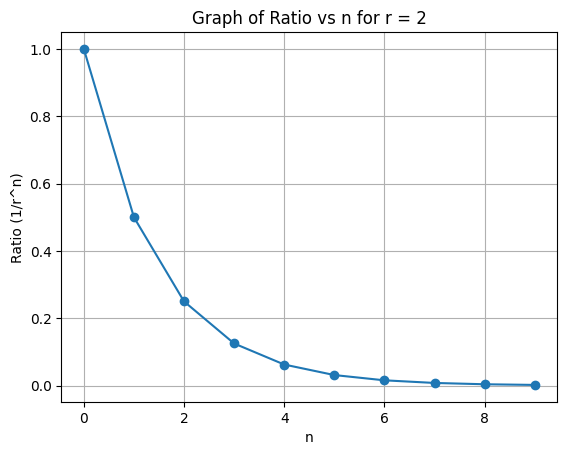
\includegraphics[width=\columnwidth]{figs/figure1}
\caption{Plot of ratio vs $1/r^n$ for r = 2}
\end{center}
\end{figure}

\end{document}